% !TEX root = ../Sesiones-TDA-Ejercicios.tex

%%%%%%%%%%%%%%%%%%%%%%%%%%%%%%%%%%%%%%%%%%%%%%%%%%%%%%%%%%%%%%%%%%%%%%%%%%%%%%%%%%%%
%%%%%%%%%%%%%%%%%%%%%%%%%%%%%%%%%%%%%%%%%%%%%%%%%%%%%%%%%%%%%%%%%%%%%%%%%%%%%%%%%%%%
\chapter{Python y PyCharman}

\etocsetnexttocdepth{3}
\etocsettocstyle{\hrule \vskip 0.15cm \subsubsection*{Índice Parcial}\vskip 0cm}{\vskip 0.15cm\hrule}
\localtableofcontents

\

\


\formatoNormal


%%%%%%%%%%%%%%%%%%%%%%%%%%%%%%%%%%%%%%%%%%%%%%%%%%%%%%%%%%%%%%%%%%%%%%%%%%%%%%%%%%%%
%%%%%%%%%%%%%%%%%%%%%%%%%%%%%%%%%%%%%%%%%%%%%%%%%%%%%%%%%%%%%%%%%%%%%%%%%%%%%%%%%%%%
\section{Introducción}

\cm[red]{Python} es un lenguaje de programación de propósito general escrito sobre el lenguaje C. Se usa en una amplia variedad de disciplinas como biología, finanzas, química, análisis numérico, inteligencia artificial, etc. También se usa como lenguaje script para los administradores de sistemas informáticos.

En esta primera sesión práctica se indica cómo llevar a cabo las instalaciones de \cm[red]{Python} y algunas herramientas, cuáles son los pasos usuales de una sesión de trabajon así como los pasos a realizar para documentar nuestros programas.


%%%%%%%%%%%%%%%%%%%%%%%%%%%%%%%%%%%%%%%%%%%%%%%%%%%%%%%%%%%%%%%%%%%%%%%%%%%%%%%%%%%%
%%%%%%%%%%%%%%%%%%%%%%%%%%%%%%%%%%%%%%%%%%%%%%%%%%%%%%%%%%%%%%%%%%%%%%%%%%%%%%%%%%%%
\section{Instalación de Python}


 \key{CPython} es la implementación estándar de Python. {\small \url{https://www.python.org/}}
	\begin{itemize}
	\item CPython no traduce el código \cm[red]{Python} a C por sí mismo.  
	\item Ejecuta un intérprete. 
	\item Instalación básica $\approx$ 120Mb
	\item Cython es un módulo que compila a código en C o C++ desde Python
		\begin{itemize}
		\item Permite incluir C en código Python
		\item Permite incluir \cm[red]{Python} en código C y ser compilado.
		\end{itemize}
	\end{itemize}
	

Puede instalar \cm[red]{Python} (\key{CPython} ) sin problema en su Sistema Operativo:

	\begin{itemize}
	\item 
	Windows. Consulte \url{https://www.python.org/downloads/windows/}. Durante la instalación, verá una ventana de <<Setup>>. Asegúrate de marcar las casillas <<Add Python xx to PATH>> o <<Add Python to your environment variables>>

Para más detalles consultar \- \url{https://tutorial.djangogirls.org/es/python_installation/}
	
	\item 
	mac OS.   Descargue e instale (como en Windows) pero \textbf{tenga mucho cuidado} \textbf{si su SO es anterior al 2022}. Algunos macOS llevan Python como parte del sistema operativo. Trabajar directamente sobre Python del SO puede conllevar que éste deje de funcionar si no se sabe exactamente qué se está haciendo. 
	
	Si tiene un Mac OS, abra un terminal y ejecute \texttt{python --version}. Si como resultado obtiene \texttt{Python 2.xx} entonces debe instalar previamente Homebrew y después \cm[red]{Python} de Homebrew.
		\begin{enumerate}
		\item Para instalar Homebrew, abra un terminal y ejecute:
		
		$ $ \hbox{\small \texttt{ruby -e "}\verb+$+\texttt{(curl -fsSL https://raw.githubusercontent.com/Homebrew/install/master/install)"}}
		
		\item Inserte el directorio de Homebrew al inicio de tu variable de ambiente PATH. Puedes hacer esto agregando la siguiente línea al final de tu archivo \verb+~/.profile+ o \verb+~/.bash_profile+
\begin{verbatim}
export PATH=/usr/local/bin:/usr/local/sbin:$PATH
\end{verbatim}


		\item Instalar Python 3: \texttt{brew install python3}
		\end{enumerate}
		
		Ahora tendrá dos versiones de Python. La del SO y la ubicada en \texttt{/usr/local/Cellar}.
		
		Ahora bien, si al ejecutar \texttt{python --version} \/ obtiene un mensaje de error, entonces solo debe instalar la distribución de la página oficial: \url{https://www.python.org/downloads/}
		
		
%		Otra opción es usar \cm{pyenv} si ya tiene instalada otra versión de Python:
%
%$ $ \hbox{\small \url{https://stackoverflow.com/questions/62898911/how-to-downgrade-python-version-from-3-8-to-3-7-mac}}
		
	\item GNU/Linux
		\begin{description}
		\item[\tt Debian:] \verb+sudo apt install python3+
		\item[\tt Fedora:] \verb+sudo dnf install python3+
		\end{description}
	\end{itemize}
	
	
Como alternativa a CPython (la distribución estándar) puede instalar Python usando alguna suit especializada que lo incluya.

Quizás la más conocida sea  \key{Anaconda Python.} Desarrollada por Anaconda. {\small \url{https://www.anaconda.com/}}
	\begin{itemize}
	\item Pensada para desarrolladores/empresas de \cm[red]{Python} que necesiten respaldo.
	\item Es una distribución pensada para ciencia de los datos y aprendizaje automático que incluye Python, IPython y R entre otros.
	\item Orientado el trabajo comercial y científico. 
	\item La más completa para ciencias de los datos. 
	\item La edición individual es gratis. Otras superan las \$10mil.
	\item Instalación básica $\approx$ 4.8Gb. CPython+Editores+IDE+...
	\item Gestiona paquetes \cm[red]{Python} y de terceros.
	\end{itemize} 
Existe una versión libre y versiones comerciales. Al adaptarse desde estudiantes a profesiones, la distribución es usada por millones de usuarios. Destaca su sistema de gestión de paquetes llamado conda.

Otra suit alternativa es \key{ActivePython.} Desarrollado por Activestate. {\small \url{https://www.activestate.com/}}. Tiene la misma filosofía de Anaconda.

Otras alternativas curiosas son:
\begin{itemize}
\item \key{PyPy.} Alternativa a CPython. \url{https://www.pypy.org/}
	\begin{itemize}
	\item  Compilador JIT\footnote{Compilación en tiempo de ejecución (JIT) mejora el rendimiento compilando a bytecode y traducir el bytecode a código máquina nativo en tiempo de ejecución. } de RPython.
	\item 4.2 veces más rápido que CPython.
	\item Usa el ``núcleo'' de CPython.
	\end{itemize}
	
\item \key{IronPython.} Alternativa a CPython. \url{https://ironpython.net/}
	\begin{itemize}
	\item Implementado en C\#.
	\item Integra \cm[red]{Python} en .NET\footnote{Plataforma de aplicaciones que permite la creación y ejecución de servicios web y aplicaciones de Internet.}.
	\item Ejecuta \cm[red]{Python} en Microsoft DLR (entorno de ejecución)
	\end{itemize}

\item \key{Jython.} Alternativa a CPython. \url{https://www.jython.org/}
	\begin{itemize}
	\item Implementado en Java.
	\item En Java se pueden añadir librerías de Jython.
	\item En Jython se puede añadir java.
	\item Ejecuta \cm[red]{Python} en JVM.
	\end{itemize}

\item Hay más: WinPython, MicroPython, Pycopy, RustPython, MesaPy, ...
\end{itemize}




%%%%%%%%%%%%%%%%%%%%%%%%%%%%%%%%%%%%%%%%%%%%%%%%%%%%%%%%%%%%%%%%%%%%%%%%%%%%%%%%%%%%
%%%%%%%%%%%%%%%%%%%%%%%%%%%%%%%%%%%%%%%%%%%%%%%%%%%%%%%%%%%%%%%%%%%%%%%%%%%%%%%%%%%%
\section{Instalación de Herramientas de Desarrollo}


Existen varios Entornos de Desarrollo Integrado (Integrated Development Environment, IDE) y editores que ayudan a la programación. En el contexto de \cm[red]{Python} podemos destacar
\begin{itemize}
\item PyCharm. Es uno de los IDE de \cm[red]{Python} más completos \url{http://jetbrains.com/pycharm}

\item PyDev. Un buen IDE con soporte para CPython, Jython e Iron Python. \url{http:// pydev.org}

\item Spyder. IDE de código abierto y totalmente gratuito. Desarrollado principalmente para científicos e ingenieros. Se recomienda usar el que viene con Anaconda \url{https://www.spyder-ide.org/}

\item Visual Studio Code. Es un editor de código fuente con multitud de plugins. \url{https://code.visualstudio.com/} 

\item Sublime Text. Es un editor que viene con muchas opciones. \url{https://www.sublimetext.com/}

\item Atom. Otro editor. Es de lo más usados. \url{https://atom.io/}
\end{itemize}


Veamos cómo instalar algunos de ellos.


%%%%%%%%%%%%%%%%%%%%%%%%%%%%%%%%%%%%%%%%%%%%%%%%%%%%%%%%%%%%%%%%%%%%%%%%%%%%%%%%%%%%
\paragraph{Instalación de PyCharm}

\begin{enumerate}
\item Instalar \cmbox{PyCharm Community} desde \url{https://www.jetbrains.com/es-es/pycharm/download/}
\item Para instalar un diccionario español:
		\begin{itemize}
		\item Descargar en cualquier directorio el diccionario \\
		\url{https://github.com/EOM/Spell-Checking-PHPStorm-Spanish-dic-UTF8/blob/master/spanish-utf8.dic}.
		\item Desde PyCharm seleccionar \menu[>]{Preferences > Editor > Natural Languages > Spelling} y  añadir el diccionario anterior.
		\end{itemize}
		
\item En \menu[>]{PyCharm > Preferences > Plugins} instalarás complementos que te pueden ser útiles. En particular, algunos tema para el IDE:
		\begin{itemize}
		\item Godot Theme (recomendado)
		\item Theme Collection
		\item Visual Studio Code Dark Plus Theme
		\end{itemize}

	Pulsar \keys{Apply}
\item En \menu[>]{PyCharm > Preferences > Editor > Proofreading}
	\begin{itemize}
	\item Seleccionar \keys{\mbox{+}$_\downarrow$}
	\item Seleccionar \menu{Español}
	\end{itemize}
	Pulsar \keys{Apply}
\end{enumerate}


Para el desarrollo de las prácticas de este curso de Tecnología de la Programación es suficiente PyCharm Community, que es la que está instalada en los ordenadores de la universidad. Pero también se puede descargar la versión profesional en el mismo enlace. 

Las diferencias entre una y otra versión se pueden ver la final de la página \url{https://www.jetbrains.com/es-es/pycharm/features/}. De la versión profesional os puede venir bien la "Capacidad para desarrollo remoto". Esta característica permite que todos los miembros de un grupo puedan desarrollar código a la vez, lo que es ideal para esta primera parte de las prácticas de la asignatura.

El problema está en que PyCharm Professional vale la friolera de unos cuantos cientos de dólares pero si eres estudiante te lo dan gratis. 
Solo tienes que seguir los pasos que se indican en \url{https://www.jetbrains.com/es-es/community/education/#students}.
Si quieres, puedes solicitar la licencia rellenado los datos y pon como año de graduación 3 o 4 más del año actual. Recibirás un correo de ``JetBrains account''.  Sigue las instrucciones del correo y recibirá un correo de “JetBrains sales” para activar tu paquete gratuito donde debes pulsar ``click this link''. Echo todo esto, solo debes entrar en tu cuenta de JetBrains y descargar PyCharm Professional. Una vez instalado, inicia tu cuenta desde el propio programa para obtener el ``code with me''\footnote{Estos pasos fueron facilitados por el alumno Pablo Roques Villa durante el curso 2021-2022}. 


%%%%%%%%%%%%%%%%%%%%%%%%%%%%%%%%%%%%%%%%%%%%%%%%%%%%%%%%%%%%%%%%%%%%%%%%%%%%%%%%%%%%
\paragraph{Instalación de Spyder}

\begin{enumerate}
\item Puede instalar el IDE desde Anaconda. Siga los pasos para ese entorno. 
\begin{itemize}
\item Si usa Linux, la recomendación es usar Anaconda, \url{https://docs.spyder-ide.org/current/installation.html#anaconda-install-ref}, aunque puede seguir los pasos que se indican para instalarlo directamente en el sistema.
\end{itemize}

\item Alternativamente puede instalar el IDE desde la opción \textsc{Download} de \url{https://www.spyder-ide.org/}
\begin{itemize}
\item En Windows, si aparece un cuadro de diálogo SmartScreen, haga clic en \textit{More Info} seguido de \textit{Run away} y luego continúe con los pasos del instalador.

\item Si al arrancar Spyder obtiene este error: 

\centerline{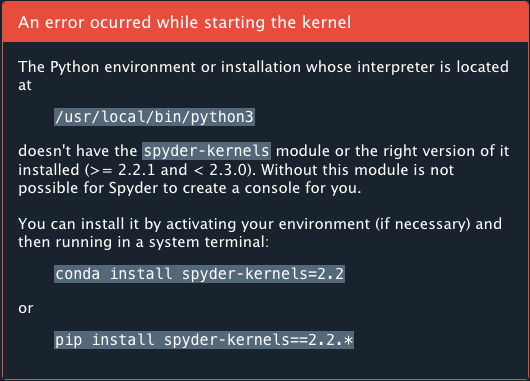
\includegraphics[width=.5\textwidth]{error-spyder}}

deberá de instalar spyder-kernels (p.e. \texttt{pip3 install spyder-kernels==2.2.1}). Los kernels instalarán los paquetes ipython (shell python interactivo), jupyter  (notebooks), pygments (coloreado de sintaxis), tornado (servidor web) y otros paqeutes que permitirán dar mayor funcionalidad a Spyder.

Si usa Anaconda, no debería presentar este error, pero si instaló Python en su SO y debe instalarlo, conviene usar un entorno virtual y no trabajar directamente sobre la versión Python del SO. No obstante, esta tarea puede ser muy difícil en algunos sistemas como maxOS (p.e. la versión homebrew no funciona en Mojave).

\end{itemize}


\end{enumerate}



%%%%%%%%%%%%%%%%%%%%%%%%%%%%%%%%%%%%%%%%%%%%%%%%%%%%%%%%%%%%%%%%%%%%%%%%%%%%%%%%%%%%
\paragraph{Instalación de Visual Studio Code y Plugins}


\begin{enumerate}
\item Instalar el editor desde \url{https://code.visualstudio.com/}

\item En el menú de la izquierda seleccionar Extensions y a continuación buscar la extensión \cm[red]{Python}.

\item Instalar el extensión \key{Python de Microsoft} y a continuación pulsar \menu{Reload}.

\item Instale también la extensión \key{Pylance} para mejorar la extensión anterior. Vuelva a recargar.

\item Abrir la paleta de comandos \keys{\cmd}+\keys{\shift}+\keys{P} o \keys{\ctrlwin}+\keys{\shift}+\keys{P} y teclear \key[orange]{Shell Command: Install 'code' command in PATH} con lo que tendremos el comando nuevo \key[blue]{code} en nuestra sistema operativo.

\item En la parte inferior izquierda aparece la versión del interprete \key[red]{Python} que se está utilizando. Se puede cambiar haciendo click para a continuación seleccionar la versión de \key[red]{Python} deseada.

\item Como plugins complementarios, instalar:
	\begin{itemize}
	\item \key{vscode-icons} de VSCode Icons Team (recomendado)
	\item \key{Python DocString Generator} de Nils Werner
	\item \key{AI Python Docstring Generator} Tae Hwan Jung
	\item \key{Python Preview} de dongli
	\item \key{PlantUML} de jebbs
	\item \key{Markdown Preview Enhanced} de Yiyi Wang
	\item \key{Visual Studio IntelliCode} de Microsoft
	\item \key{VSC-Prolog} de arthurwang
	\end{itemize}
	
\end{enumerate}




%%%%%%%%%%%%%%%%%%%%%%%%%%%%%%%%%%%%%%%%%%%%%%%%%%%%%%%%%%%%%%%%%%%%%%%%%%%%%%%%%%%%
%%%%%%%%%%%%%%%%%%%%%%%%%%%%%%%%%%%%%%%%%%%%%%%%%%%%%%%%%%%%%%%%%%%%%%%%%%%%%%%%%%%%

\section{Sesión de trabajo} \label{sec:sesionTrabajo}


\subsection{Usando Editores}

Siga siempre los siguientes pasos para trabajar un proyecto desde su inicio:

\begin{enumerate}
% - - - - - - - - - - - - - - - - - - - - - - - - -
\item \textbf{Creación del directorio principal del proyecto.} Esto se hace una vez.

 Construya una carpeta donde vaya a guardar todo los referente a su proyecto \cm[red]{Python}. 
 Aquí se guardará tanto los ficheros fuentes como la documentación del proyecto.
Llamaremos \directory{Proyecto} a esta carpeta pero en la práctica pon un nombre significativo al proyecto que vayas a desarrollar.


% - - - - - - - - - - - - - - - - - - - - - - - - -
\item \textbf{Creación del entorno virtual.} Esto se hace una vez.

Con  \key[red]{Python 3} se suministra el módulo \cmbox{venv} que permite crear entornos virtuales con la siguiente instrucción (se hace una vez):
\begin{Verbatim}
$ python3 -m venv venv
\end{Verbatim}

Con lo que tendremos esta nueva estructura de directorios
\directory{Proyecto > venv}  

% - - - - - - - - - - - - - - - - - - - - - - - - -
\item \textbf{Activación del entorno virtual.} 

Para poder usar el ambiente hay que activarlo. La instrucción es levemente diferente dependiendo del sistema operativo

\begin{itemize}
\item UN*X
\begin{Verbatim}
$ source venv/bin/activate
\end{Verbatim}

\item Windows

\begin{Verbatim}
$ source venv/Scripts/activate  % Si usa bash
$ venv/Scripts/activate  % Si usa cmd
\end{Verbatim}
\end{itemize}

Entonces el nombre del ambiente virtual aparecerá en el prompt. 

% - - - - - - - - - - - - - - - - - - - - - - - - -

\item \textbf{Trabajar sobre el proyecto.} 

Activado el entorno virtual puede trabajar exactamente igual que si estuviera en el entorno general. Podrá utilizar un editor de código cualquiera con el que escribir sus programas y ejecutarlos
\begin{Verbatim}
$ python3 Proyecto/main.py
\end{Verbatim}

También podrá instalar tantos paquetes como requiera su proyecto 
\begin{Verbatim}
$ pip3 install paquete
\end{Verbatim}
todos se guardarán en \directory{Proyecto > venv} y no le afectará a otras librerías de otros proyectos.

% - - - - - - - - - - - - - - - - - - - - - - - - -
\item \textbf{Desactivar el ambiente virtual.} 

Cuando finalice, vuelva al ambiente \cm[red]{Python} general que tenga por defecto su sistema. Para ello desactive el ambiente actual.
\begin{Verbatim}
$ deactivate
\end{Verbatim}

\end{enumerate}
% - - - - - - - - - - - - - - - - - - - - - - - - -



%%%%%%%%%%%%%%%%%%%%%%%%%%%%%%%%%%%%%%%%%%%%%%%%%%%%%%%%%%%%%%%%%%%%%%%%%%%%%%%%%%%%
%%%%%%%%%%%%%%%%%%%%%%%%%%%%%%%%%%%%%%%%%%%%%%%%%%%%%%%%%%%%%%%%%%%%%%%%%%%%%%%%%%%%

\subsection{Sesión de Trabajo con PyCharm} \label{subsec:SesionPyCharm}
Cuando se trabaja con ciertos IDEs los pasos anteriores se realizan con unos pocos clicks de ratón.


\begin{enumerate}
% - - - - - - - - - - - - - - - - - - - - - - - - -
\item \textbf{Creación del directorio principal del proyecto, creación del directorio del proyecto fuente y activación del entorno virtual} 

\begin{itemize}
\item Seleccionar \menu{File > New Project}

\item En la nueva ventana, en la opción \menu{Location} pinchar sobre el icono \directory{\mbox{}} 
	\begin{itemize}
	\item Seleccionar la carpeta donde crearás todos tus proyectos.\\
			En su caso selecciona \keys{New Folder}. 
	\item Cuando termine seleccionar  \keys{Open}
	\end{itemize}

	Supondremos que la carpeta se llama \directory{Proyecto}.
	
\item En la misma ventana considere la opción \menu{New environment} 
	\begin{itemize}
	\item Seleccione el valor \cmbox{Virtualenv}
	\item En la opción \menu{Location} 
		\begin{itemize}
		\item Pinchar sobre el icono \directory{\mbox{}}
		\item Selecciona \keys{New Folder} y crea el directorio para el entorno virtual.\\
				Supongamos que se llama \directory{venv}
		\item Seleccionar  \keys{Open}
		\end{itemize}
	\end{itemize}
	
\item En la misma ventana, asegúrese que está activa la opción \menu{Create a main.py}.
\item Seleccionar  \keys{Create}.
\item En su caso, seleccionar \menu{Open Proyect} con \keys{New Windows}.
\end{itemize}

Cuando finalice estos pasos se creará un nuevo proyecto donde verá el siguiente contenido:
\begin{itemize}
\item[] \directory{Proyecto/venv}
\item[] \directory{Proyecto/main.py}
\end{itemize}


% - - - - - - - - - - - - - - - - - - - - - - - - -
\item \textbf{Trabajar sobre el proyecto.} 

En \directory{Proyecto} deberá crear todo su código fuente. De todos los ficheros habrá uno que se llamará \mbox{\directory{main.py}} que será el módulo principal - lo construyó antes ¿recuerda? Lo verá también porque en la barra superior aparece precisamente el nombre \cmbox{main$\bigtriangledown$}

Para ejecutar el proyecto puede usar estas alternativas.
	\begin{itemize}
	\item Pinche sobre \cmboxb[green!75]{\mbox{ $\blacktriangleright$ }} en la barra superior
	\item Pinche sobre \cmboxb[green!75]{\mbox{ $\blacktriangleright$ }} en el editor, en la linea donde aparezca \pyv{if __name__ == '__main__':}
	\item Seleccione \menu{Run > Run 'main'}
	\end{itemize}
	
\item \textbf{Desactivar el ambiente virtual.} 

La versión más sencilla de esta acción es cerrar el proyecto.

\end{enumerate}
% - - - - - - - - - - - - - - - - - - - - - - - - -



%%%%%%%%%%%%%%%%%%%%%%%%%%%%%%%%%%%%%%%%%%%%%%%%%%%%%%%%%%%%%%%%%%%%%%%%%%%%%%%%%%%%
%%%%%%%%%%%%%%%%%%%%%%%%%%%%%%%%%%%%%%%%%%%%%%%%%%%%%%%%%%%%%%%%%%%%%%%%%%%%%%%%%%%%
\section{Documentar el Código del Proyecto} % https://martinber.github.io/guia-sphinx/introduccion.html#estructura
\label{sec:documentarCodigo}

Documentar un programa es escribir las especificaciones de las abstraciones implementadas. Consiste en añadir información en el código fuente. Se realiza en forma de comentarios (docstrings) para explicar qué es lo que hace para que los usuarios programadores de su programa entiendan su funcionamiento. Además, como ayuda a su entendimiento permite detectar errores y extender el programa para tenga nuevas funcionalidades. Todo programa tiene errores (es cuestión de tiempo) y todo programa que tenga éxito será modificado en el futuro, por lo que la documentación es un paso fundamental.


Los programas en Python se documentan con tres comillas dobles o con la almohadilla. Las tres comillas se usan como docstring (para las definiciones de las clases y las especificaciones de los métodos junto con las aclaraciones sobres los mismos). La \# se usa para hacer comentarios entre líneas del código no trivial (no para comentar todo lo que se hace).


Para documentar el proyecto con PyCharm con docstrings debe seguir los siguientes pasos

\begin{enumerate}

\item Determinar cuál será el formato del Docstring.
	\begin{itemize}
	\item \menu{PyCharm > Preferences > Tools > Python Integrated Tools}
	\item Seleccionar en \menu{Docstring} el formato \keys{reStructuredText}.
	\end{itemize}

\item Construir los docstring de cada función. 

El docstring es una especificación informal de la función. Consta de un pequeño resumen del objetivo de la función, una breve descripción de los parámetros de entrada y de salida. Para construirlos en PyCharm basta empezar una nueva línea con 3 dobles comillas \cmbox[red!70]{"\/"\/"\/}    justo después de la signatura de la función, pulsar \keys{\return} y completar la información. 

Un ejemplo de docstring es el siguiente:

\begin{pyverbatim}
def check_fin(mensaje):
    """
    Realiza una pregunta de confirmación. 
    Se dan dos opciones 1 y 2 en el mensaje de entrada.

    :param mensaje: El mensaje de la pregunta
    :return: True si se eligió 1, False en otro caso.
    """
    return '1' == input(f"{mensaje}\n1. sí\n2. no\n")
\end{pyverbatim}

\end{enumerate}

En el caso de querer indicar también el tipo de dato de los parámetros y retorno, deberá seguir los siguientes pasos:


\begin{enumerate}

\item Ir a la opción \menu{PyCharm > Preferences > Editor > General > Smart Keys > Python}

\item Seleccionar \menu{Insert type placeholders in ...}

\item Confirmar \keys{OK}
\end{enumerate}


Con esto es suficiente para que, durante el proceso de programación, pueda consultar la especificación de la función/método sin necesidad de ir a la parte del módulo donde escribió el docstring. Si escribe una función documentada y coloca el cursor del ratón sobre el nombre de la función recién escrito verá su docstring.




%%%%%%%%%%%%%%%%%%%%%%%%%%%%%%%%%%%%%%%%%%%%%%%%%%%%%%%%%%%%%%%%%%%%%%%%%%%%%%%%%%%%
%%%%%%%%%%%%%%%%%%%%%%%%%%%%%%%%%%%%%%%%%%%%%%%%%%%%%%%%%%%%%%%%%%%%%%%%%%%%%%%%%%%%
\section{Generar la Documentación de un Proyecto} % https://martinber.github.io/guia-sphinx/introduccion.html#estructura


En ocasiones nos interesa tener un documento completo con todas las especificaciones de todas las funciones para poder hacer un estudio más concienzudo de las funcionalidades. Comentemos varias formas para hacer esto.
 



%%%%%%%%%%%%%%%%%%%%%%%%%%%%%%%%%%%%%%%%%%%%%%%%%%%%%%%%%%%%%%%%%%%%%%%%%%%%%%%%%%%%
%%%%%%%%%%%%%%%%%%%%%%%%%%%%%%%%%%%%%%%%%%%%%%%%%%%%%%%%%%%%%%%%%%%%%%%%%%%%%%%%%%%%
\subsection{Sin crear ficheros externos}
% - - - - - - - - - - - - - - - - - - - - - - - - -

\cm[red]{Python} incorpora \cmbox{pydoc} para visualizar todos las funciones y clases de su proyecto.
Teclee lo siguiente en el terminal.

\begin{Verbatim}
$ cd Proyecto   # Confirme que se encuentra en el proyecto con ficheros .py
$ python3 -m pydoc -p 2334
$ Server commands: [b]rowser, [q]uit
server> b
\end{Verbatim}

Se abrirá un navegador y podrá consultar la documentación. Para terminar escriba {\tt q}.
\begin{Verbatim}
$ Server commands: [b]rowser, [q]uit
server> b
server> q
\end{Verbatim}



%%%%%%%%%%%%%%%%%%%%%%%%%%%%%%%%%%%%%%%%%%%%%%%%%%%%%%%%%%%%%%%%%%%%%%%%%%%%%%%%%%%%
%%%%%%%%%%%%%%%%%%%%%%%%%%%%%%%%%%%%%%%%%%%%%%%%%%%%%%%%%%%%%%%%%%%%%%%%%%%%%%%%%%%%
\subsection{Creando ficheros externos} En este caso es mejor usar otras herramientas como pydoctor o sphinx.
En ambos casos tendrá que realizar los siguientes pasos
% - - - - - - - - - - - - - - - - - - - - - - - - -

\begin{enumerate}[nosep]

\item Instalar los nuevos módulos en el entorno virtual.

Desde el IDE lo puede hacer en \menu{PyCharm > Preferences > Project: Nombre Proyecto > Python Interpreter}
	\begin{itemize}
	\item Asegurése de que se tiene seleccionado el intérprete del entorno virtual, en \menu{Python Interpreter}
	\item Seleccionar \keys{\mbox{+}}, buscar  \menu{pydoctor}, \menu{pdoc3} y \menu{Sphinx} e instalar los paquetes.
	\end{itemize}


Alternativamente puede abrir un terminal y con el entorno virtual activo, ejecutar
\begin{Verbatim}
$ pip3 install pydoctor
\end{Verbatim}
o bien
\begin{Verbatim}
$ pip3 install pdoc3
\end{Verbatim}
o bien
\begin{Verbatim}
$ pip3 install Sphinx
\end{Verbatim}


\item Asegúrese de que tienen esta estructura de directorios 
		\begin{itemize}
		\item[] \directory{Proyecto}, lugar donde está sus programas .py comentados con sus especificaciones.
		\item[] \directory{Proyecto/docs}, lugar donde estará toda la documentación referente a la resolución del problema (enunciados, ayudas, etc).
		\item[] \directory{Proyecto/docs/api}, el lugar donde se generará la documentación del programa. Se asume que no contiene nada.
		\end{itemize}
\end{enumerate}


%%%%%%%%%%%%%%%%%%%%%%%%%%%%%%%%%%%%%%%%%%%%%%%%%%%%%%%%%%%%%%%%%%%%%%%%%%%%%%%%%%%%
%%%%%%%%%%%%%%%%%%%%%%%%%%%%%%%%%%%%%%%%%%%%%%%%%%%%%%%%%%%%%%%%%%%%%%%%%%%%%%%%%%%%
\subsubsection{Cómo usar \texttt{pydoctor}}

Siga los siguientes pasos:
\begin{enumerate}[nosep]
	\item Teclee en el terminal
\begin{Verbatim}
$ cd Proyecto   # Asegúrese que está en el directorio del proyecto
$ touch programa/__init__.py  # Convertir el programa en módulo (importante)
$ pydoctor --make-html --html-output=docs/api --docformat=restructuredtext programa
\end{Verbatim}


	
\item Visualizar la documentación. \\
Con un navegador web abra el fichero \directory{Proyecto/docs/api/index.html}
\end{enumerate}



%%%%%%%%%%%%%%%%%%%%%%%%%%%%%%%%%%%%%%%%%%%%%%%%%%%%%%%%%%%%%%%%%%%%%%%%%%%%%%%%%%%%
%%%%%%%%%%%%%%%%%%%%%%%%%%%%%%%%%%%%%%%%%%%%%%%%%%%%%%%%%%%%%%%%%%%%%%%%%%%%%%%%%%%%
\subsubsection{Cómo usar \texttt{pdoc3}}

Sigue los pasos de \texttt{pydoctor}. Solo tienes que cambiar la línea de comandos para generar la documentación.

\begin{Verbatim}
$  pdoc3 --html --output-dir html programa
\end{Verbatim}




%%%%%%%%%%%%%%%%%%%%%%%%%%%%%%%%%%%%%%%%%%%%%%%%%%%%%%%%%%%%%%%%%%%%%%%%%%%%%%%%%%%%
%%%%%%%%%%%%%%%%%%%%%%%%%%%%%%%%%%%%%%%%%%%%%%%%%%%%%%%%%%%%%%%%%%%%%%%%%%%%%%%%%%%%
\subsubsection{Cómo usar \texttt{sphinx}}

Se presenta a continuación un resumen de los que puede encontrar en el siguiente vídeotutorial:

\hfil
\url{https://youtube.com/playlist?list=PL__ig9hYf07AdLfTOMrWwSvYeUdWUY3Zt}

También dispones del paquete {\tt documentationPythonProject.zip} en el aula virtual para que sigas los pasos del tutorial.

Los pasos a seguir son:

\begin{enumerate}[nosep]
\item Teclee en el terminal
\begin{Verbatim}
$ cd Proyecto/doc/api   # Asegúrese que está en el directorio doc/api del proyecto
$ sphinx-quickstart
\end{Verbatim}

Para Mac: Si al ejecutar \cmbox{sphinx-quickstart} diera problemas, deberá seguir los siguientes pasos:
\begin{Verbatim}
$ open /usr/local/bin/sphinx-quickstart -a textedit
cambiar la primera línea por #!/usr/local/bin/python3
Archivo > Guardar
Archivo > Cerrar 
\end{Verbatim}



\item Introducir los siguientes datos:
	\begin{itemize}[nosep]
	\item \cm[magenta]{Separar directorios fuente y compilado (y/n) [n]:} \keys{Enter}
	\item \cm[magenta]{Nombre del proyecto:} Pon un nombre adecuado \keys{Enter}
	\item \cm[magenta]{Autor(es):} Pon tu nombre \keys{Enter}
	\item \cm[magenta]{Liberación del proyecto []: } \keys{Enter}
	\item \cm[magenta]{Lenguaje del proyecto [en]:]} \cm{es} \keys{Enter}
	\end{itemize}

Se habrá generado el siguiente contenido en \directory{Proyecto > doc > api}:

\begin{Verbatim}
Makefile
_build
_static
_templates
conf.py
index.rst
make.bat
\end{Verbatim}

\item Editar el fichero \cmbox{conf.py} 

\begin{itemize}
\item Descomentar las siguientes líneas:
\begin{Verbatim}
# import os
# import sys
# sys.path.insert(0, os.path.abspath('.'))
\end{Verbatim}

y de la tercera, cambiar \cmbox{'.'} por \cmbox{'../..'} para referenciar a \directory{Proyecto} (lugar donde están los fuentes \cmbox{.py}).

\item Además, añadir la siguiente extensión (con comillas simples):
\begin{Verbatim}
extensions = ['sphinx.ext.autodoc']
\end{Verbatim}
\end{itemize}


\item Editar el fichero \cmbox{index.rest} y adaptarlo a tu gusto. Lo más básico sería poner \cmbox{modules}:
\begin{Verbatim}
.. toctree::
   :maxdepth: 2
   :caption: Contents:

   modules
\end{Verbatim}

Puede cambiar los valores de \texttt{caption} y \texttt{maxdepth} si lo desea.

\item Ejecutar en el directorio \cmbox{docs/api} la instruccion \cmbox{sphinx-apidoc -o . ../..}

Lo que indica esta instrucción es que busque de forma recursiva en \cmbox{../..} (directorio \directory{Proyecto}) todos los módulos y paquetes de \cm[red]{Python} y cree un archivo reST por cada uno de ellos en el directorio \cmbox{.} (directorio  \directory{Proyecto/doc/api}).

\item Por último generamos la documentación. En UN*X
\begin{Verbatim}
make html
\end{Verbatim}
Para Windows use \cmbox{make.bat}


\item Visualizar la documentación. \\
Con un navegador web abra el fichero \directory{Proyecto/docs/api/\_build/\_static/index.html}
\end{enumerate}

\

Opcionalmente puede cambiar la estética de la documentación. 

\begin{enumerate}[nosep]
\item En su entorno virtual ejecute \cmbox{pip3 install sphinx\_rtd\_theme} para instalar uno de los muchos temas disponibles.
\item Edite \cmbox{conf.py}
\item Cambie la entrada \cmbox{html\_theme = 'sphinx\_rtd\_theme'}
\item Genere de nuevo la documentación.
\end{enumerate}

Tiene más temas en \url{https://pypi.org/search/?q=sphinx+theme&o=} pero no pierda el tiempo en la estética.



\begin{ejercicio}$ $
\begin{itemize}
\item Modifique el formato del Docstring.
	\begin{itemize}
	\item \menu{PyCharm > Preferences > Tools > Python Integrated Tools}
	\item Seleccionar en \menu{Docstring} el formato \keys{Google}.
	\end{itemize}

\item Borre el docstring de una función que tenga parámetros y valor de retorno. 

\item Vuelva a escribirlo con 3  comillas dobles \cmbox[red!70]{"\/"\/"\/}    justo después de la signatura de la función y pulse \keys{\return}.

Verá que el formato \keys{Google} es diferente al formato \keys{reStructuredText}.

\item Vuelva a generar la documentación con \cmbox{pydoctor}. 
\end{itemize}

El formato  \keys{Google} es más legible en una una documentación pero también ocupa más líneas de texto en el código lo que para funciones cortas de pocas líneas puede ser un inconveniente.
\end{ejercicio}





%%%%%%%%%%%%%%%%%%%%%%%%%%%%%%%%%%%%%%%%%%%%%%%%%%%%%%%%%%%%%%%%%%%%%%%%%%%%%%%%%%%%
%%%%%%%%%%%%%%%%%%%%%%%%%%%%%%%%%%%%%%%%%%%%%%%%%%%%%%%%%%%%%%%%%%%%%%%%%%%%%%%%%%%%
\section{Gestión de Algunos Errores en PyCharm}


\subsection{Resolver el problema de Paquetes en PyCharm}

A algunos de vosotros os ocurre que algún módulo (fichero .py) no reconoce algún otro módulo del proyecto.  Para solucionar esto sigue los siguientes pasos.

Memoriza la teoría. En las transparencias se indica que se debe tener un fichero vacío \pyv{__init__.py} para poder importar todos los módulos de una carpeta. Es decir, hay que construir un paquete con sus módulos. La construcción de paquetes desde PyCharm se hace seleccionando  \menu[>]{File > New > Python Package}. Simplemente crea un carpeta con el fichero \pyv{__init__.py}. Observa que todas las carpetas menos \directory{venv} están en el mismo color. Si además tienen un punto sobre la carpeta, entonces esa carpeta es un paquete.



En principio, solo con lo anterior deberías poder importar los módulos de los paquetes. Pero si te siguiera saliendo el mensaje \texttt{Unresolved Reference XXXX} entonces sigue los siguientes pasos:

\begin{itemize}
\item Marca el paquete como una fuente raíz. 

Pon el ratón sobre la carpeta y pulsa botón derecho del ratón. Selecciona \menu[>]{Mark Directory as > Sources Root}. La carpeta cambiará de color.


\item Añadir la nueva al \texttt{PYTHONPATH}. 

Selecciona  \menu[>]{Preferences > Build, Execution, Deployment > Console > Python Console}  y asegurarte de marcar las dos opciones de \texttt{Add content} y  \texttt{Add source}.

\item Limpia la caché y reiniciar PyCharm. Selecciona \menu[>]{File > Invalide Cache > Restart}.

\end{itemize}

Ya no deberías tener más problemas de reconocimiento de los módulos de los paquetes.

\begin{quote}
\textbf{IMPORTANTE: }

Algunos, para solucionar el problema habrán seleccionado \menu{Install and Import package} en vez de hacer la importación como se indica aquí. Si tras realizar esa acción PyCharm ha dejado de quejarse, \textbf{tienes un problema}. Habrán instalado unos paquetes extras en \directory{venv} y ahora tu program entiende que debe importar esos paquetes en vez de los que tú has desarrollado. Obviamente tendrás que quitar esos paquetes extras que no os sirven para nada en la resolución del ejercicio. 

Posiblemente alguno de ellos son: \texttt{Point}, \texttt{Agent}, \texttt{Vector}, \texttt{Vector2}, \texttt{state}, .... La forma de comprobar que has instalado unos paquetes que NO deberías de haber instalado es seleccionar \menu[>]{Preferences > Project > Python Interpeter} para ver el listado de los paquetes que has instalado. Si hay alguno cuyo nombre coincide con algunos de los nombre que te indico o con el nombre de algún módulo/clase que tú hayas construido tendrás que eliminar el paquete porque muy probablemente tu programa estará usando ese paquete en vez del tuyo.
\end{quote}
